\section{Modernisation de NTMIX et développement d'une version 3D}
\label{sec:part1}

\subsection{Travail préliminaire}
Une grande partie du temps en début du stage a été consacré à la prise en main de NTMIX. En effet NTMIX est un code d'environ 30000 lignes de codes ($\approx 25000$ + $\approx 5000$ pour CHEMKIN). Pour me familiariser avec NTMIX, j'ai utilisé Allinea DDT, un debugger. Il permet d'observer le comportement d'un programme, de voir l'ordre d'exécution des différentes fonctions, et ainsi comprendre un peu mieux son déroulement. C'est aussi durant cette période que j'ai pu discuter avec mes encadrants afin d'affiner les objectifs du stage.

\paragraph{Gestion du projet}Afin de faciliter le développement, j'ai utilisé \textit{git} un logiciel de gestion de versions. Il permet de stocker l'ensemble des fichiers modifiés en respectant la chronologie de ces changements. Il est donc possible de garder une trace de toutes les modifications réalisées sur le code original, autorisant ainsi à revenenir à une version précédente dans le cas où le code modifié serait faux.
 
\subsection{Migration de NTMIX}
Après cette période et avant de commencer à développer une version en 3 dimensions de NTMIX, j'ai dû moderniser le code. En effet, NTMIX a été développé en Fortran 77 ce qui ne permettait pas l'allocation dynamique de tableau; l'ensemble des variables étaient allouées de manière statique ce qui augmentait la taille de l'exécutable et réduisait grandement la flexibilité; en effet, il était nécessaire de recompiler le programme à chaque changement de la taille du maillage. Pour résoudre ce problème, il m'a été demandé de migrer le code du standard Fortran 77 au standard Fortran 90.

\subsubsection{Réécriture de code}Cette partie consistait donc à réécrire le code dans une norme plus récente. Une majorité des modifications étaient liées à la syntaxe du code. Pour rendre la tâche plus aisée, j'ai utilisé des expressions régulières; ce sont des séquences de caractères qui définissent des motifs de recherche et qui sont particulièrement utiles pour remplacer un motif par un autre. Par exemple, en Fortran 77, le \textit{C} ou \textit{c} placé en début de ligne indique le début d'un commentaire, mais en Fortran 90 c'est un \textit{!} qui a cet usage. La figure \ref{fig:regex} montre une expression utilisée pour modifier ces commentaires dans le code.

\begin{figure}[ht]
  \centering
  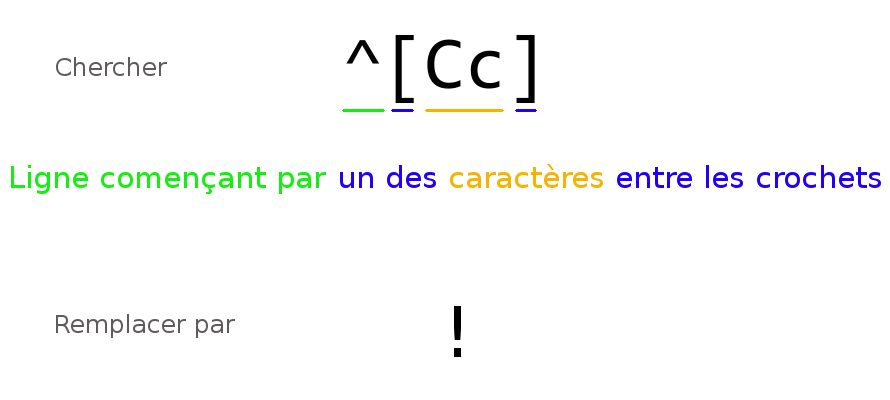
\includegraphics[scale=0.3]{figures/regex.png}
  \caption{\label{fig:regex}Exemple d'expression régulière}
\end{figure}

% Exemple ^#.*?"\(.*?\)\.com"

L'utilisation de ces expressions m'a donc permis de gagner beaucoup de temps et de m'éviter une tâche fastidieuse.

\subsubsection{Gestion de la mémoire}En Fortran, les blocs COMMON permettent de définir des zones mémoires globales, accessibles depuis n'importe où dans le code. Le problème est qu'il faut répliquer ce bloc à chaque endroit du code où les variables qu'il contient doivent être utilisées, le plus souvent avec des instructions non-standard du Fortran. Un autre problème est qu'il faut définir la taille des tableaux contenus dans ces blocs à la compilation, ce qu'y va à l'encontre de mon objectif. Pour pallier ces problèmes, ces blocs ont été transformés en modules (introduits en Fortran 90) qui permettent également d'avoir une zone de mémoire globale mais les tailles des tableaux peuvent être précisées à l'exécution.

\subsubsection{Post-traitement}NTMIX génère des fichiers binaires contenant l'état physique de la simulation à un instant donné. Un programme annexe à NTMIX permettait de transformer ces fichiers en fichiers pouvant être visualisés grâce à Plot3D. Ce code ne fonctionnant plus, il a été modifié pour génèrer des fichiers HDF5 (\textit{Hierarchical Data Format}), un format très répandu dans la communauté CFD, qui permettent de structurer de grandes quantités de données. La figure \ref{fig:hdf5_struct} montre un exemple d'entête de fichier HDF5 généré par l'application; les ensembles X,Y et Z contiennent les coordonnées des points du domaine de calcul dans des tableaux monodimensionnels dont le type est précisé (ici des nombres à virgule flotante de 64 bits) et les autres ensembles de données contiennent les valeurs des différentes variables de la simulation (ici dans dans des matrices).

\begin{figure}[!ht]
  \centering
  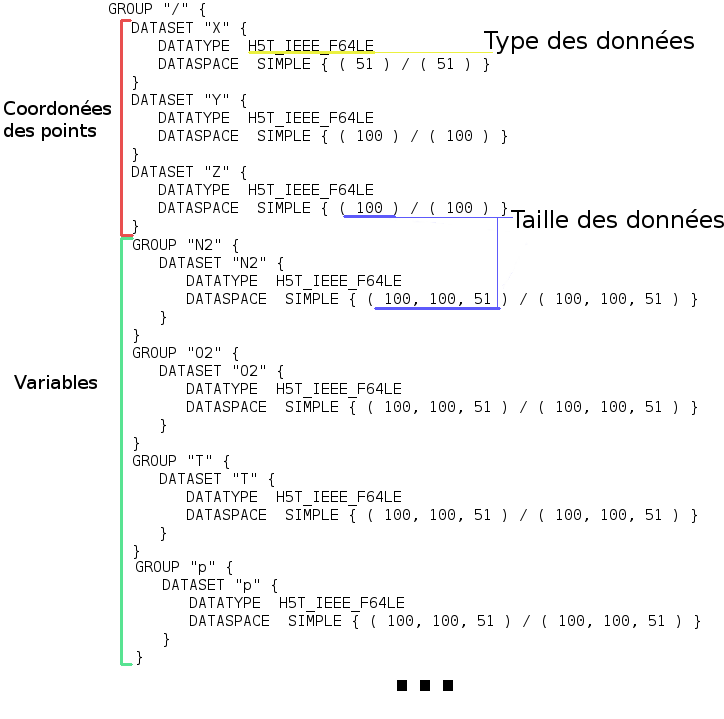
\includegraphics[scale=0.5]{figures/hdf5_struct.png}
  \caption{\label{fig:hdf5_struct} Structure d'un fichier HDF5}
\end{figure}

Cependant, ces fichiers ne peuvent être directement lus par un logiciel de visualisation, j'y ai donc joint des fichiers XDMF (\textit{eXtensible Data Model and Format}). Ce format a été développé pour le calcul haute performance et notamment pour permettre la visualisation des données par des logiciels comme ParaView ou EnSight. Il permet de définir un maillage et une topologie d'un domaine grâce aux coordonnées des points présentes dans le fichier HDF5. Les valeurs des variables seront ensuite lues depuis les différents ensemble de données présents dans le fichier HDF5 et associées au point du maillage correspondant.



\begin{figure}[!ht]
  \centering
  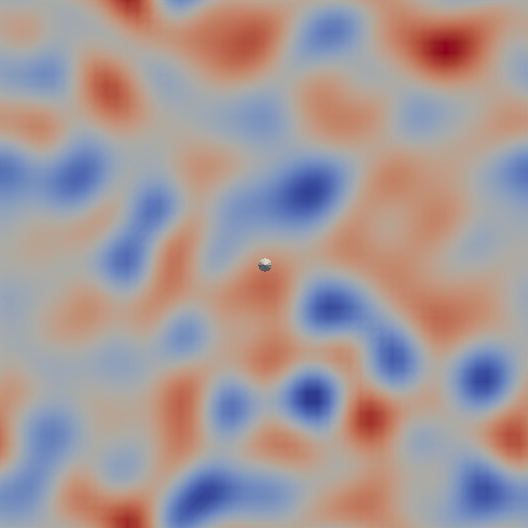
\includegraphics[scale=0.3]{figures/thi-example.png}
  \caption{\label{fig:visu}Exemple de visualisation, Turbulence Homogène isotrope - ParaView}
\end{figure}

% \begin{itemize}
% \item Changement de syntaxe
% \item Changement des bloc commom en modules
% \item Changement des equivalence en pointeur
% \item Allocation dynamique des tableaux
% \item Utilisation de namelist pour changer la taille du maillage et certains paramètres du problème physique.
% \end{itemize}


\subsubsection{Validation}
Pour vérifier que les modifications réalisées ne changeaient pas le comportement du programme, j'ai écrit un script permettant de comparer les résultats fournis par ma version avec ceux du programme initial. Ce script génère des fichiers d'initialisation de NTMIX avec différentes configurations du domaine (permettant ainsi de s'assurer que toutes les régions du code soient exécutées). Le script lance ensuite le programme initial et la version modifiée avec ces fichiers puis compare les résultats obtenus par chacune des versions.


\paragraph{}Avec l'apparition de l'allocation dynamique, beaucoup de problèmes peuvent apparaître; mémoire non désallouée entrainant des fuites de mémoires (pouvant entrainer une saturation de la mémoire de la machine ainsi qu'un plantage du code), erreur sur les tailles des tableaux entraînant des erreurs de segmentation (tentative d'accès à des zones mémoire n'appartenant pas au programme).
J'ai donc utilisé Valgrind, un outil permettant notamment d'analyser la mémoire d'un programme durant son exécution autorisant ainsi à vérifier l'apparition de tels problèmes.




\subsection{Passage en 3D}

\subsubsection{Méthode}\label{sec:3dmeth}
Plusieurs parties du code prévoyaient déjà le passage du code en 3 dimensions, ainsi la préparation des tableaux utilisés pour le calcul des gradients, le traitement des cas réactifs ainsi que le stockage des données nécessaires aux calculs des conditions limites étaient présents. La librairie CHEMKIN utilisée pour les calculs des cinétiques complexes est adimensionnée ce qui a permis d'ajouter une dimension sans avoir à modifier la totalité de la librairie. Ces points ont facilité le passage de l'application en 3D.


\paragraph{}Même avec les points précédents, beaucoup de modifications étaient nécessaires avant d'obtenir une version 3D fonctionnelle. Pour minimiser les erreurs pouvant être induites par ce changement, j'ai dans un premier temps décidé de laisser la nouvelle dimension à une taille de 1. En effet, si la dimension ajoutée est de 1, le programme doit avoir un comportement identique à la version 2D. Les variables conservatives de la simulation (densité, vitesses, énergie..) étaient toutes représentées par des tableaux en 2 dimensions. J'ai donc progressivement remplacé ces tableaux par d'autres en 3D, toujours avec la dernière dimension de taille 1,  me permettant ainsi de vérifier les résultats obtenus tout au long du développement. Lorsque je remplaçais ces tableaux, je modifiais en même temps les nombreuses boucles de calcul parcourant ceci (un parcours sur X et Y devient un parcours sur X,Y et Z). Une fois ces modifications terminées, et le comportement du programme validé, j'ai augmenté la taille de la troisième dimension et me suis intéressé aux problèmes suivants.

%1/sqrt(1)*exp(-((coordsX/(2*sqrt(1)))^2))

\subsubsection{Calcul des gradients}%Les gradients indiquent la façon dont les grandeurs physiques (densité, vitesse, énergie, etc.) évoluent au cours du temps. Maintenant que la 3ème dimension était différente de 1, il était nécessaire que les calculs des gradients soient modifiés. Ces calculs s'effectuaient sur un plan; il a donc fallu les modifier pour qu'ils prennent en compte tout l'espace. Il a fallu également ajouter les calculs de gradients selon l'axe Z.

Les gradients permettent de calculer l'évolution spatiale des grandeurs physiques (densité, vitesse, énergie, etc.). Le gradient pour une fonction bidimensionnelle $f(x,y)$ était donc décrit comme suit:
$$\nabla f(x,y) =\left(\frac{\partial f}{\partial x}(x,y),\frac{\partial f}{\partial y}(x,y)\right) $$

En 3D, les fonctions devant être dérivées sont dépendantes de $(x,y,z)$, les dérivées se réalisent maintenant sur un espace et non plus sur un plan:
$$ \nabla f(x,y,z) =\left(\frac{\partial f}{\partial x}(x,y,z),\frac{\partial f}{\partial y}(x,y,z)\right)$$


Il existe plusieurs dérivées selon les conditions aux frontières de la simulation (périodique, apériodique, symétrique); pour chacune de ces méthodes de dérivation, il a fallu ajouter les calculs de $\frac{\partial f}{\partial z}$ qui n'étaient pas présent dans cette version de NTMIX ce qui amène à la version finale du calcul des gradients:

$$ \nabla f(x,y,z) =\left(\frac{\partial f}{\partial x}(x,y,z),\frac{\partial f}{\partial y}(x,y,z),\frac{\partial f}{\partial z}(x,y,z)\right)$$



\subsubsection{Conditions limites}\label{sec:nsbc}
Une simulation DNS doit être très précise et ne fournit pas de moyen de minimiser la création d'ondes d'instabilités numériques qui se propagent ensuite dans le domaine, sont réfléchies aux frontières et peuvent générer de nouvelles ondes physiques\cite{baritaud1996direct}. Ce procédé entraîne l'apparition d'oscillations non-physiques qui faussent les résultats de la simulation. Pour pallier ce problème, il est courant de supprimer les conditions aux frontières en utilisant un domaine de calcul périodique. Mais dans le cas de l'étude des écoulements réactifs, il est nécessaire de traiter les frontières. Pour résoudre ce problème, la méthode NSCBC (\textit{Navier-Stokes Characteristic Boundary Conditions}) est utilisé dans NTMIX. J'ai donc dû implémenter la version 3D de cette méthode à l'aide des équations fournies par Poinsot et Lele (1992)\cite{POINSOT1992104}. Les équation \textit{NSCBC} sur la direction $x$ pour un cas tridimensionnel sont présentées en annexe \ref{app:nscbc}. 



Dans la version 2D, l'équation (\ref{eq:l3}) n'était pas présente car $w$ (la vitesse sur l'axe Z n'existait pas) et a donc dû être ajouter. En 3D, les équations (\ref{eq:l2}) et (\ref{eq:l3}) changent selon la direction (ex: lorsqu'on est sur la dimension $y$, $\mathcal{L}_2 = v \frac{\partial u}{\partial y}$ et $\mathcal{L}_3 = v \frac{\partial w}{\partial y}$ avec $u,v$ et $w$ les champs des vitesses selon les axes $x,y$ et $z$.

\subsubsection{Initialisation}Il a également été nécessaire de modifier certaines fonctions d'initialisation afin qu'elles prennent en compte la 3ème dimension. Je n'ai pas modifié toutes les nombreuses fonctions d'initialisation mais seulement celles permettant de lancer les tests présentés dans la section suivante.




% \begin{itemize}
% \item Changement de la taille des tableaux
% \item Ajout de la vitesse sur l'axe Z
% \item Ajout des conditions limites sur Z
% \item Modification du calcul des dérivées
% \item Modification du calcul de l'énergie cinétique: $\rho_e = \rho\frac{1}{2}(u^2+v^2+w^2)$
% \end{itemize}

\subsubsection{Validation}\label{sec:3D-validation}
Comme dit précédemment (sec. \ref{sec:3dmeth}), j'ai d'abord testé le comportement du programme 3D en précisant la 3ème dimension à 1 ce qui m'a permis de comparer les résultats avec la version 2D. Plusieurs tests m'ont ensuite été suggérés pour valider le comportement en 3 dimensions de NTMIX:

\begin{itemize}
\item Écoulements uniformes: un flux uniforme traverse le domaine selon un axe; le flux étant constant, les dérivées doivent rester nulles et les vitesses ne doivent pas varier
\item Un front de flamme (une zone dans laquelle se déroule la combustion):
  \begin{itemize}
  \item Vitesse nulle: le front de flamme doit rester statique et un phénomène de diffusion doit être observé (mouvement de molécules d'une région de haute concentration vers une région de faible concentration)
  \item Vitesse non-nulle: en plus du phénomène de diffusion, la convection doit également apparaître (mouvement de groupe de molécules au sein d'un fluide)
  \end{itemize}
\item Turbulence homogène isotrope
\end{itemize}

\paragraph{Écoulements uniformes}
Comme dit précédemment, les dérivées doivent être nulles dans ce cas et la simulation doit donc rester dans son état initial. Comme on peut le voir sur la figure \ref{fig:uniform_flow}, les vitesses selon les 3 axes sont restées constantes au cours du temps.
 
%\begin{figure}[ht]
%  \centering
%  % \includegraphics[scale=0.3]{figures/uniform_flow.png}
%  \caption{\label{fig:uniform_flow}Ecoulement uniforme}
%\end{figure}

\paragraph{Front de flamme}
Un cas simple a été utilisé pour ce front de flamme; 2 espèces chimiques et la concentration d'une espèce est modélisée par une gaussienne centrée simplifiée en $e^{-(x^2)}$ et l'autre par $1-e^{-(x^2)}$ permettant ainsi d'avoir une concentration totale de 1 en tout point du domaine. Pour observer l'effet de diffusion, nous utilisons la fonction dérivée d'une gaussienne: $f(x,t)=\frac{1}{t}e^{f}$. Sur la figure \ref{fig:diff}, nous pouvons observer en bleue la valeur initiale d'une espèce, en vert sa valeur au temps $t$ de la simulation et en rouge la valeur théorique.

% $f(x,t_0)=e^{\frac{-(x-x_0)^2}{\sigma^2}}$
% \begin{figure}[ht]
%   \centering
%   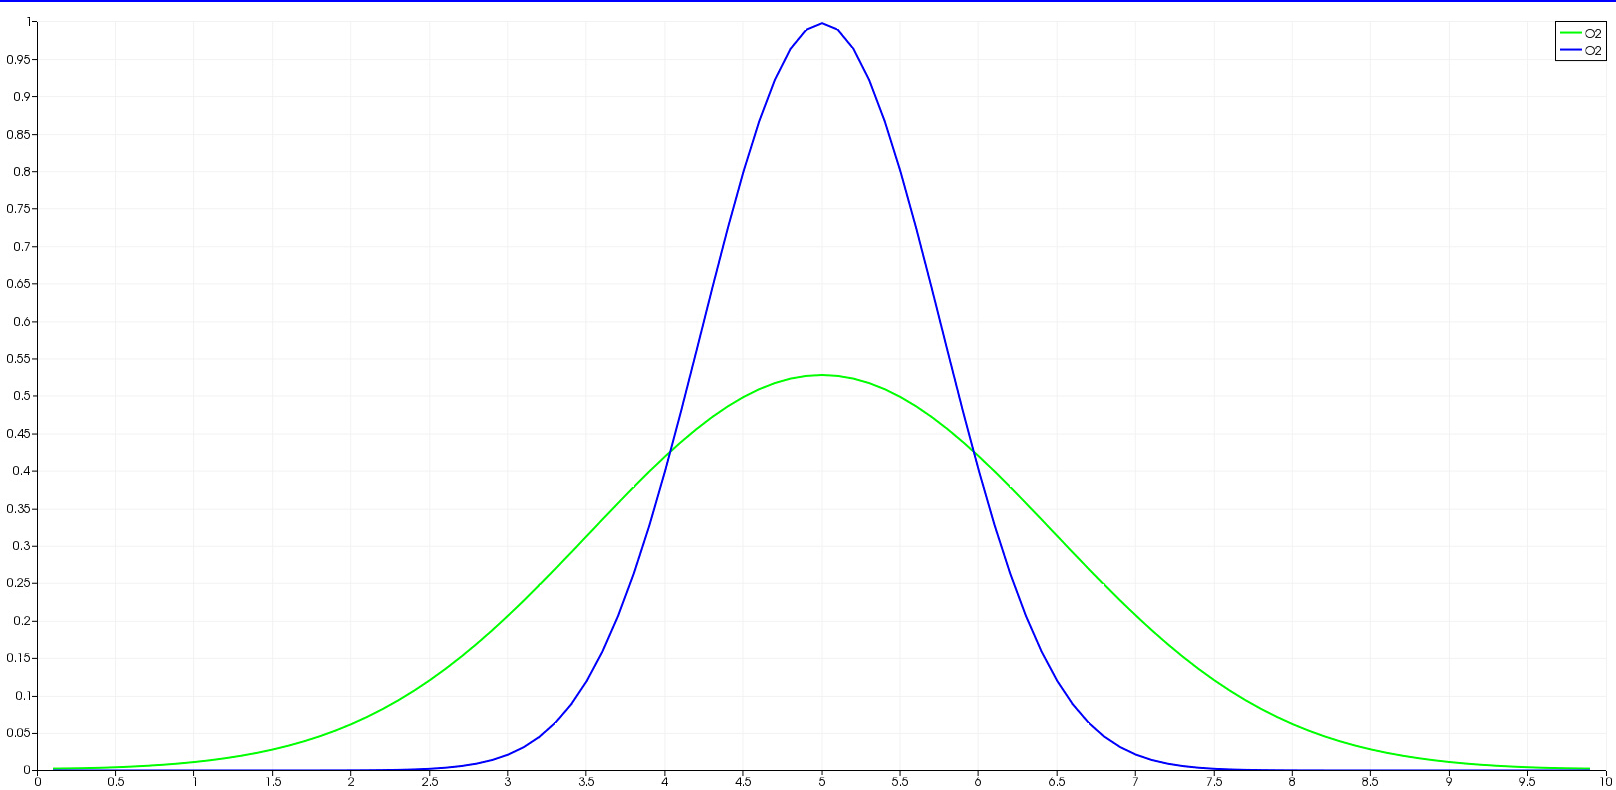
\includegraphics[scale=0.15]{figures/diff.png}
%   \caption{\label{fig:diff} }
% \end{figure}

%\begin{figure}[t!]
%  \centering
%  \begin{subfigure}[b]{0.5\textwidth}
%    \centering
%    %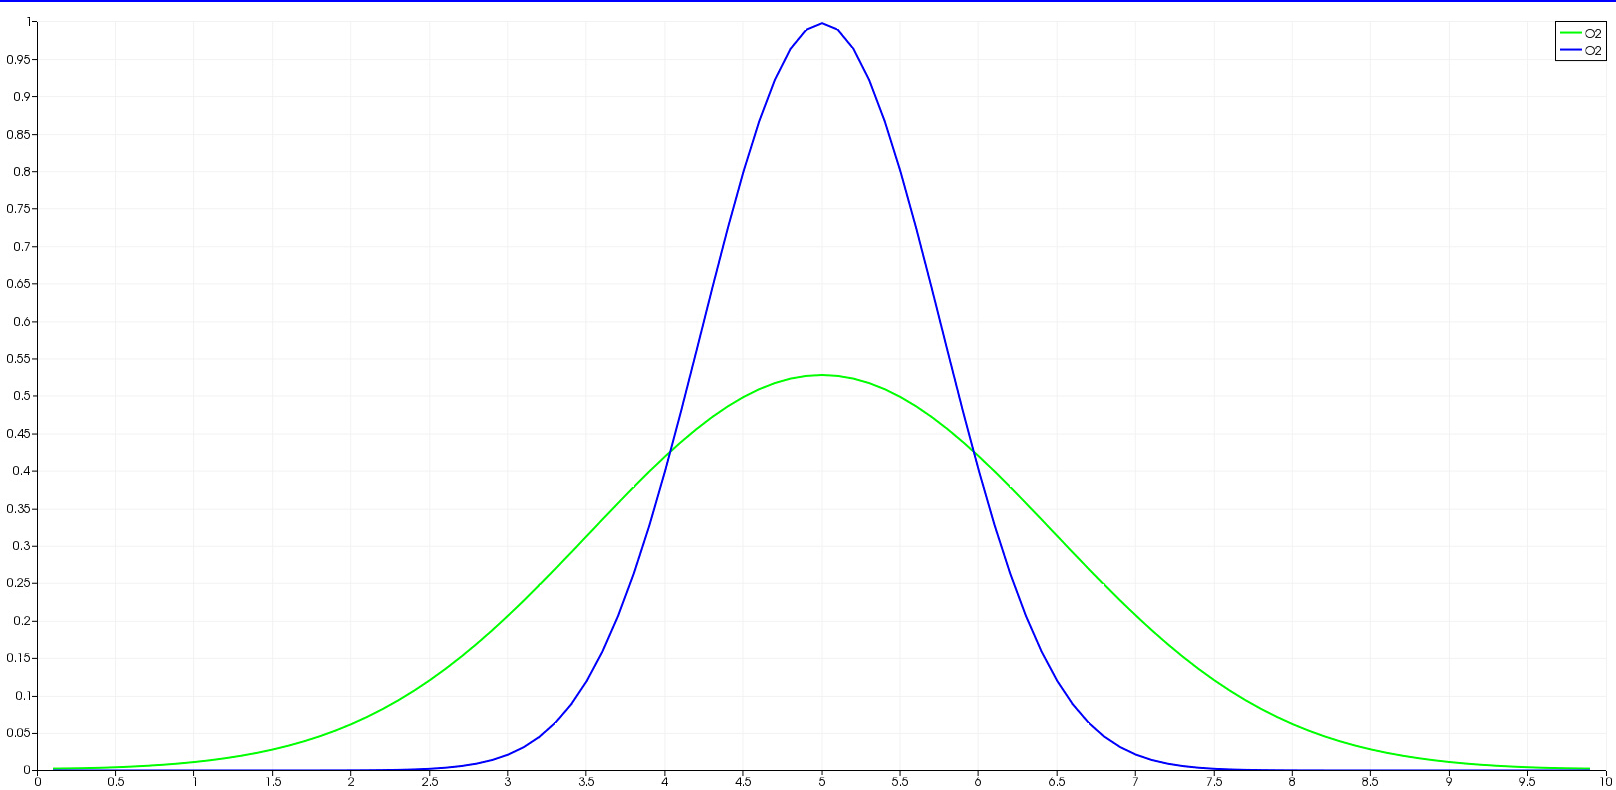
\includegraphics[width=.9\linewidth]{figures/diff.png}
%    \caption{\label{fig:diff_0}Valeur x $t_0$}
%  \end{subfigure}%
%  ~ 
%  \begin{subfigure}[b]{0.5\textwidth}
%    \centering
%    %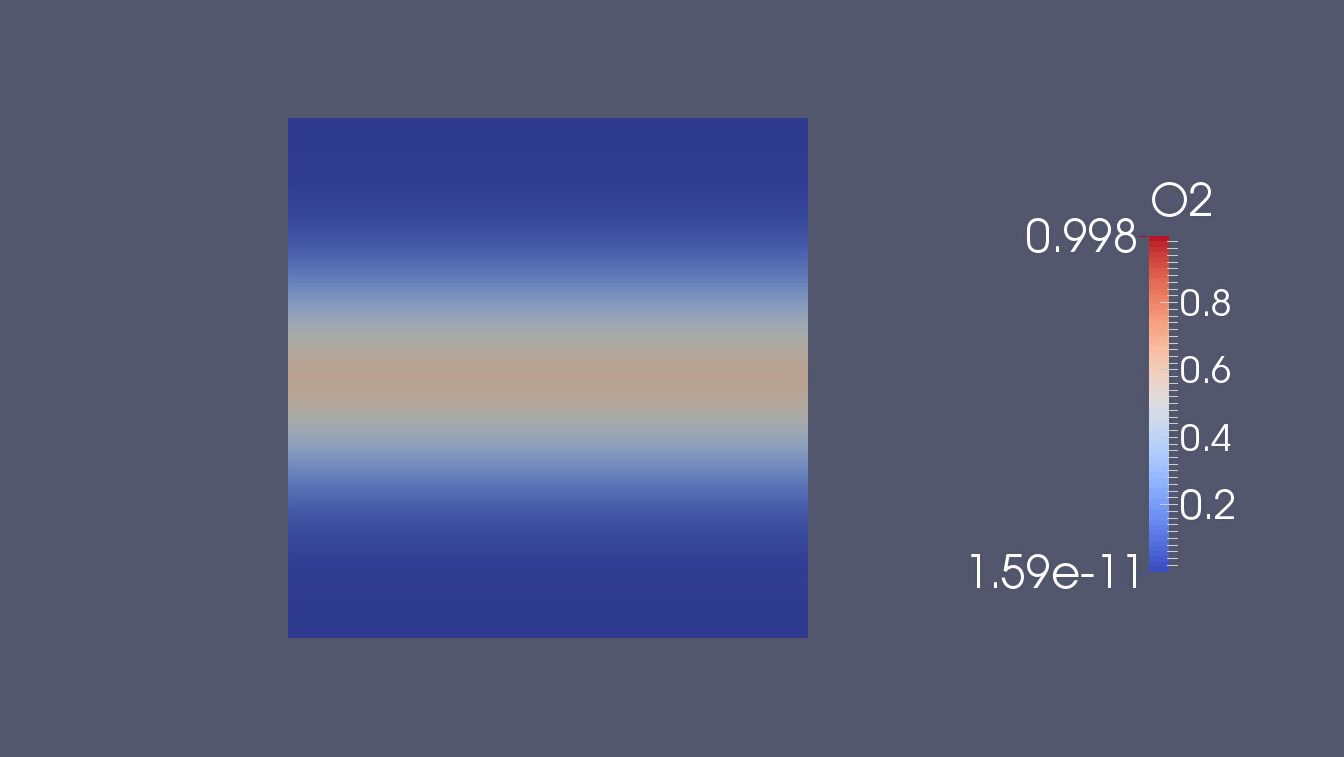
\includegraphics[width=.9\linewidth]{figures/diff_325.png}
%    \caption{\label{fig:diff_325}Valeur x $t$}
%  \end{subfigure}
%  \caption{Caption place holder}
%  \centering
%  \begin{subfigure}[b]{0.5\textwidth}
%    \centering
%    %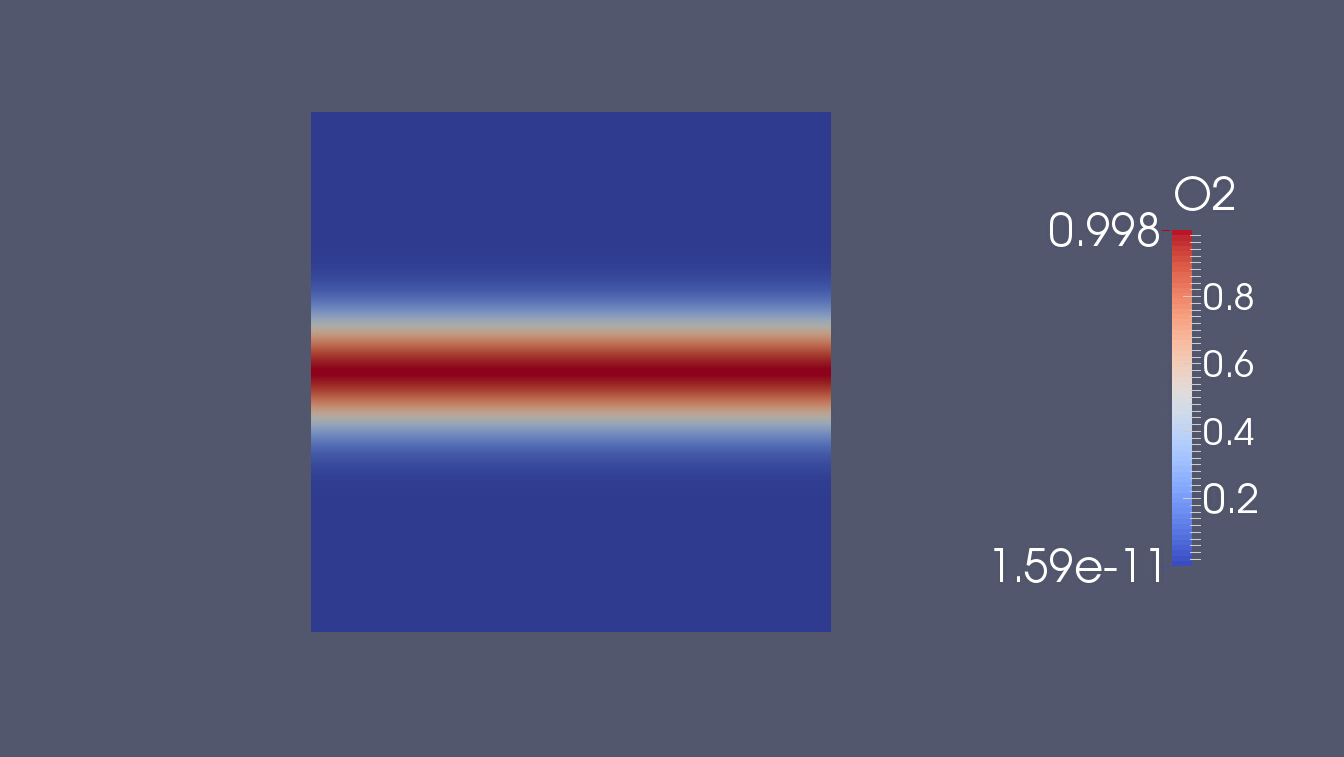
\includegraphics[width=.9\linewidth]{figures/diff_0.png}
%    \caption{\label{fig:diff_0_domain}Valeur x $t_0$ - Domaine complet}
%  \end{subfigure}%
%  ~ 
%  \begin{subfigure}[b]{0.5\textwidth}
%    \centering
%    %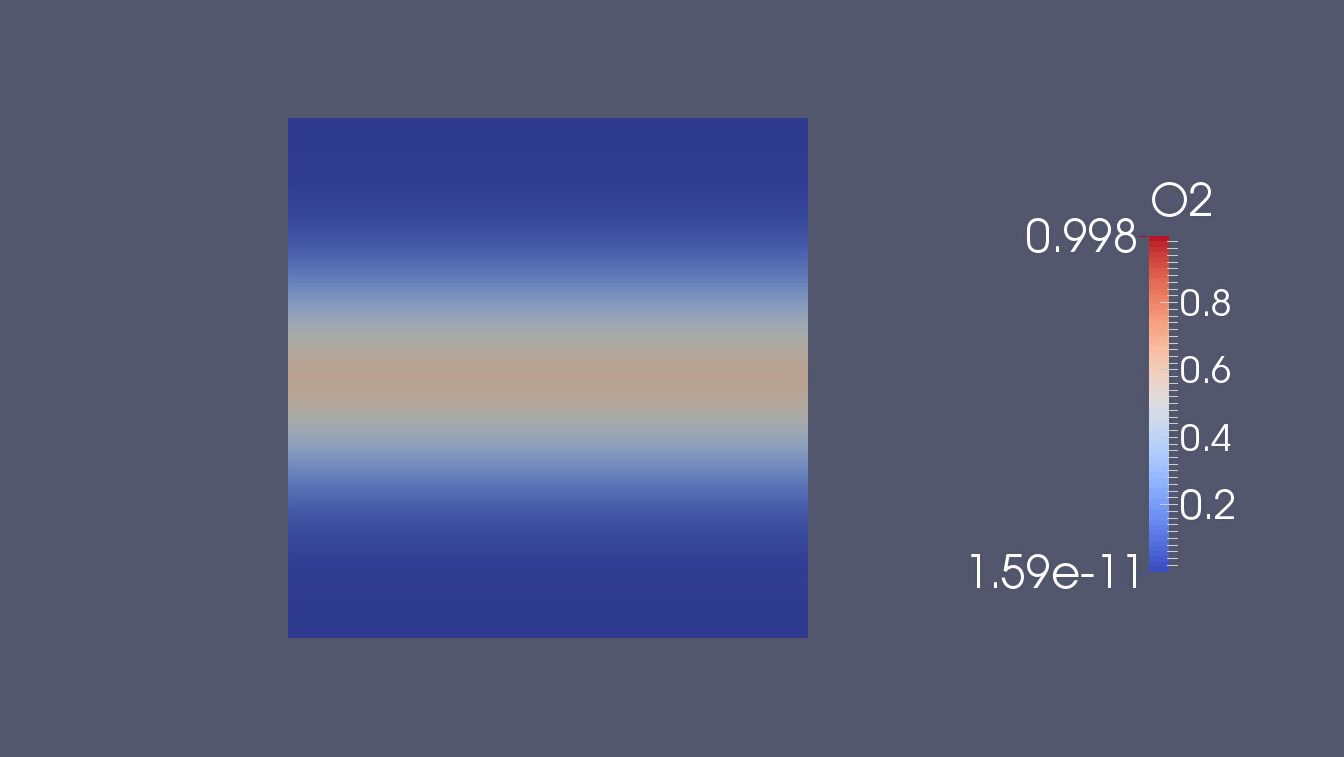
\includegraphics[width=.9\linewidth]{figures/diff_325.png}
%    \caption{\label{fig:diff_325_domain}Valeur x $t$ - Domaine complet}
%  \end{subfigure}
%  \caption{\label{fig:diff_}Diffusion}
%\end{figure}



\paragraph{Turbulence homogène isotrope}Ce cas de test est moins trivial que les autres. Il simule cette fois-ci un flux turbulent (un flux dans lequel la vitesse varie en tous points, de manière imprévisible). Homogène et isotrope se rapporte à certaines caractéristiques d'un tel flux. 

%\begin{figure}[ht]
%  \centering
%  %\includegraphics[scale=0.3]{figures/turbiso.png}
%  \caption{\label{fig:turbiso}Turbulence homogène isotrope}
%\end{figure}



